\section{QuickDough Framework}\label{sec:framework}
QuickDough is an FPGA loop accelerator generation framework. It generates FPGA accelerators for
compute intensive loop kernels in the order of seconds through the use of an SCGRA overlay. It also
generates the drivers of the accelerators automatically, integrating both software and hardware
generation in a unified framework.

\subsection{QuickDough Overview}
\figref{fig:framework} illustrates the proposed FPGA loop accelerator design framework named QuickDough.
It roughly consists of a conventional software compilation path, a fast and common FPGA loop accelerator
generation path and a slow yet rare accelerator library update path. The first path of QuickDough is to compile
the overall software application to the host processor after replacing the compute kernels with
calls to the accelerator drivers which mainly control and transfer data to and from the accelerator. 

\begin{figure}[bt]
    \center{\includegraphics[width=0.8\linewidth]{framework}}
    \caption{QuickDough: FPGA loop accelerator design framework using 
        SCGRA overlay. The compute intensive loop kernel of an 
        application is compiled to the SCGRA overlay based FPGA
    accelerator while the rest is compiled to the host processor.}
    \label{fig:framework}
\end{figure}

The second path of QuickDough is a rapid and common route for loop accelerator generation. To begin,
the compute intensive loop kernel is statically transformed to the corresponding data flow graph
(DFG) with specified loop unrolling factor. Then the accelerator selection process selects an
accelerator from a pre-built accelerator library based on the scheduling performance and the
communication overhead. The scheduling performance is obtained from the SCGRA scheduling
process which schedules the generated DFG to the SCGRA overlay included in the selected accelerator.
The communication overhead is obtained through a communication estimation based on
the communication requirements and on-chip buffer size. After the accelerator selection
process, the specified accelerator on-chip buffer is decided and the accelerator drivers can be
generated accordingly. Meanwhile, the selected pre-built accelerator and the corresponding
scheduling result are integrated to create the final FPGA configuration bitstream. This bitstream, in
combination with the software created in the first path, forms the final application that will be
executed on a target CPU-FPGA system.

The third path of QuickDough is to update the accelerator library upon users' 
request. Users may simply provide the hardware resource budget. 
Then target operations to be supported will be decided automatically by analyzing
the DFGs produced by the DFG generator. With the resource budget and the supported 
operation set, a set of accelerator HDL models will be generated by utilizing the 
overlay template. Finally, the accelerator HDL models are implemented on target 
FPGA platforms and further updated to the accelerator library.

\subsection{SCGRA overlay based FPGA accelerator}
The QuickDough overlay consists of an array of simple processing 
elements (PEs) connected by a direct network executing 
synchronously as shown in \figref{fig:scgra-accelerator}.
Each PE computes and forwards data in lock steps, allowing deterministic 
multi-hop data communication that overlaps with computations.
The action of each PE in each cycle is controlled by an instruction 
ROM that is populated with instructions generated by the design framework.
Finally, a data memory is featured on each PE to serve as a temporary 
storage for run-time data that may be reused in the same PE or be 
forwarded in subsequent steps.

\begin{figure}[tb]
    \center{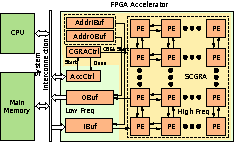
\includegraphics[width=0.65\linewidth]{scgra-accelerator}}
    \caption{SCGRA Overlay Based FPGA Accelerator}
    \label{fig:scgra-accelerator}
\end{figure}

\begin{figure}[tb]
\center{\includegraphics[width=0.65\linewidth]{pe}}
\caption{Fully pipelined PE structure. Each PE can be connected to at most 4 neighbours.}
\label{fig:pe}
\end{figure}

\begin{figure}[tb]
\center{\includegraphics[width=0.65\linewidth]{alu-v2}}
\caption{The QuickDough ALU. It supports up to 16 fully pipelined 3-input operations.}
\label{fig:ALU}
\end{figure} 

Communication between the accelerator and the host processor is 
carried through a pair of input/output buffers.
Accesses to these I/O buffers from the SCGRA array take place in 
lock step with the rest of the system.
The exact buffer location to be accessed is control by the 
AddrIBuf and AddrOBuf blocks. Both of them are ROM populated with 
address information generated from the QuickDough compiler.

\subsubsection{PE template}
\figref{fig:pe} shows the current implementation of a QuickDough 
PE template that features an optional load/store path. 
At the heart of the PE is an ALU, which is supported by a multi-port 
data memory and an instruction memory.
Three of the data memory's read ports are connected to the ALU as inputs, 
while the remaining ports are sent to the output multiplexors for 
connection to neighboring PEs and the optional store path to 
OBuf external to the PE. At the same time, this data memory takes 
input from the ALU output, data arriving from neighboring PEs, as well 
as from the optional IBuf loading path.
The action of the PE is controlled by the AddrCtrl unit that reads from the instruction memory.
Finally, a global signal from the AccCtrl block controls the start/stop of all PEs in the array.

\subsubsection{ALU template}
At the heart of the proposed PE is the ALU and it can easily be 
customized with different operations specifically for any given user 
applications. \figref{fig:ALU} shows the ALU template used 
in the QuickDough overlay. These operators in the ALU may execute 
concurrently in a pipelined fashion and must complete in a 
deterministic number of cycle. Given the deterministic nature of 
the operators, the QuickDough scheduler will 
ensure that there is never conflict at the output multiplexor.

\subsection{Loop execution on the accelerator}
The loop kernels are mostly partially unrolled, transformed to DFG and scheduled to the SCGRA
overlay of the accelerator. A straightforward way to complete the whole loop computation on top of the SCGRA
overlay is to repeat the same DFG computation until the end of the loop. Nevertheless, this may
require data transfer between host processor and I/O buffer for each DFG computation. As a result,
the communication cost increases dramatically especially when the amount of each data transfer is
small. Worse still, input data of the consecutive DFGs may be reused and the straightforward
data transfer strategy may greatly increase the total amount of data transfer through out the loop
computation. 

To alleviate this problem, we have proposed to batch data transfers for multiple executions of the
same DFG into groups as shown in \figref{fig:blocking-and-dfg-gen}. Specifically, after the loop is
unrolled $U$ times, $G$ of them are grouped together for each data transfer. This group strategy
helps to amortize the initial communication cost between host processor and the accelerator. In
addition, it allows input data to be reused for different DFG computation in the same group and the
group size is mainly limited by the I/O buffer depth. Meanwhile, the accelerator communicates with
host processor for each group execution, and thus the accelerator drive that handles the communication
depends on the I/O buffer depth as well. Clearly, accelerator with larger I/O buffer is
preferable when the rest part of the accelerator configuration fulfills the requirements. 


\begin{figure}
\center{\includegraphics[width=0.75\linewidth]{dfg-gen}}
\caption{Loop execution on an SCGRA overlay based FPGA accelerator}
\label{fig:blocking-and-dfg-gen}
\end{figure}


\subsection{FPGA loop accelerator generation}
The FPGA loop accelerator generation path is a common path and is critical for QuickDough to produce
FPGA loop accelerator rapidly. The major processes on the path are detailed in this section.

\subsubsection{DFG generation}
In order to produce an FPGA loop accelerator using SCGRA overlay, DFGs are extracted from the kernel
that is often expressed as inner loop body. The users may further unroll the loops multiple times to
increase the amount of operation parallelism in the generated DFG. In this work, we have developed a
C++ library to help automate the DFG generation with specified loop unrolling factor.

\subsubsection{Accelerator selection}
Accelerator selection process selects an accelerator from the accelerator library based on the
performance of the resulting accelerator which mainly depends on the computation latency and
communication latency. The computation latency of the loop kernel can be calculated using
\eqnref{eq:comp-lat} where $DFG\_Lat$ stands for the number of cycles needed to complete the SCGRA
scheduling and mostly depends on the SCGRA overlay size and $Freq$ stands for the pre-built
accelerator implementation frequency. The communication latency can be calculated using
\eqref{eq:comm-lat} where $Trans()$ represents the
data transfer latency function of the target platform and $GpIn$ and $GpOut$ represent the amount of
data transfer of a group which is determined by the capacity of the I/O buffers. 

\begin{equation} \label{eq:comp-lat}
    \footnotesize
    CompLat = DFG\_per\_Loop \times DFG\_Lat / Freq
\end{equation}


\begin{equation} \label{eq:comm-lat}
    \footnotesize
    CommLat = Gp\_per\_Loop \times (Trans(GpIn) + Trans(GpOut))
\end{equation}


In summary, the performance of the accelerator can be estimated with analytical models when the scheduling
performance is obtained through the DFG scheduling while the scheduling performance is mostly determined
by the SCGRA overlay size. The analytical estimation is fast while the scheduling process is
relatively slow. Therefore, the accelerator selection process essentially centers the SCGRA
overlay size selection and then explores all the accelerator configurations with the same SCGRA overlay size. 

To compromise the loop accelerator generation time and performance, three different levels of
accelerator selection optimization options are provided in this framework namely O0, O1 and O2
centering the SCGRA overlay size selection.
O0 doesn't provide any optimization, and it selects an accelerator with the smallest SCGRA overlay.
O1 estimates three typical accelerators with the smallest SCGRA overlay, a medium one and the
largest SCGRA overlay. Then the one that provides the best performance will be adopted. O3 explores all
the accelerators in the library and searches for the best accelerator configuration. With the
increase of the optimization level, the accelerator selection process spends more efforts in
searching the accelerator library for better performance and thus results in longer acceleration
generation time.

\subsubsection{DFG Scheduling}
When a DFG is extracted from the loop kernel, it can be then scheduled to execute on the
SCGRA overlay of the accelerator. Since the target DFGs typically include thousands of nodes, a
classical list scheduling algorithm \cite{schutten1996list} was adopted. A scheduling metric as
presented in \cite{colinheart}, considering both load balancing and communication cost was adopted
in our current implementation. 

\subsubsection{Accelerator bitstream generation}
The final step of the accelerator generation is to generate 
the instructions for each PE and the address sequences for the 
I/O buffers according to the scheduler's result, which will subsequently 
be incorporated into the configuration bitstream of the overlay produced 
from previous steps. Then we take advantage of the reconfigurability 
of SRAM based FPGAs and store the cycle-by-cycle configuration words 
using on-chip ROMs. The content of the ROMs are embedded in the 
bitstream and the \code{data2mem} tool from Xilinx \cite{data2mem} is 
used to update the ROM content of the pre-built bitstream directly. 
To complete the bitstream integration, \code{BMM} file that describes 
the organization and placements of the ROMs in the overlay is extracted 
from \code{XDL} file corresponding to the overlay implementation \cite{beckhoff2011xilinx}.
This bitstream integration process costs only a few seconds of the compilation time.

\subsection{Accelerator library update} 
Accelerator library consists of a number of pre-built SCGRA overlay based accelerators with
different configurations. It is the basis for the proposed rapid FPGA loop accelerator generation
framework. In this section, we will illustrate how the accelerator library is updated
given the hardware resource budget and target loop kernels.

Accelerator library update is essentially to pre-implement a group of SCGRA overlay based FPGA
accelerators upon users' request, which may either target a specified application or a domain of
applications. Since QuickDough design framework is developed to enhance the
designers' design productivity and to make FPGA accelerator design accessible to high-level
application designers, the library update which involves low-level overlay design and implementation
must be automated so that it will not become a new barrier to the application developers.

\figref{fig:auto-lib-gen} presents the proposed automatic accelerator library update flow. It
roughly consists of four steps i.e. DFG generation, common operation analysis, minimum accelerator
configuration set analysis, and accelerator HDL model generation and implementation. Since DFG generation
has been discussed in previous section, we will mainly detail the rest three steps in this section.
\begin{figure}
    \center{\includegraphics[width=0.45\linewidth]{lib-gen}}
\caption{Automatic SCGRA overlay based FPGA accelerator library update}
\label{fig:auto-lib-gen}
\end{figure}

\subsubsection{Common operation analysis}
Assume that the operations used to construct the DFG is up to the DFG generation process, the common
operation analysis step mainly decides the minimum operation set that is needed to support the
target applications. It is possible to co-optimize the DFG generation and common operation set
analysis, but it is beyond the discussion of this work. Currently, we just perform a union of the
operation types included in the DFGs. It is trivial, but the minimum operation set can be decided
automatically and rapidly.

\subsubsection{Minimum accelerator configuration set analysis}
Although the library can be implemented off-line, it does takes a long time to complete.
Therefore, we try to find out the minimum set of accelerator configurations that need to be
pre-implemented as the library and maintain the application coverage of the library at the same
time. 

The proposed SCGRA overlay based FPGA accelerator utilizes
block RAM to implement the instruction memory, data memory, on-chip buffer as well as the address
buffer, and block RAM is the hardware resource bottleneck. As a result, the library depends on how
the block RAM budget is allocated to different components of the accelerators. Therefore, the
minimum library can be obtained using equation \eqnref{eq:lib-gen}. $Row$ and $Col$ stand for the SCGRA
overlay size and they are integers. $IM$, $DM$, $AIOB$ and $DIOB$ stand for the instruction memory capacity,
data memory capacity, address IO buffer capacity and IO buffer capacity. They can only increase with the granularity of a primitive block RAM. $B$ stands for the user specified block RAM budget. 

\begin{equation} \label{eq:lib-gen}
    \footnotesize
    Row \times Col \times(IM + DM) + AIOB + IOB \leq B
\end{equation}

Moreover, empirical settings such as limiting data memory in each PE to a single primitive block RAM
(i.e. $DM = 1$), constraining the difference between SCGRA row size and column size (i.e. $Col \leq
Row \leq (Col + Gap)$, $Gap$ is an integer) and setting $AIOB = IOB$ are employed to further reduce the number of
accelerators pre-built in the library. Eventually, the accelerators in the library differ on $Row$,
$Col$, $IM$ and $IOB$. 

\subsubsection{Accelerator HDL model generation and implementation}
With the proposed SCGRA overlay template and the accelerator configurations to be pre-built in the
library, corresponding HDL models of the SCGRA overlay based FPGA accelerators are generated with a
python script. Then the library can be implemented using the conventional hardware implementation
tools. The lengthy implementations can be done in parallel. Moreover, the regular tiling structure
even allows the implementations to be accelerated using macro based implementation techniques as
presented in \cite{ROB2014}, which can be up to 20X faster than a standard HDL implementation with
negligible timing and overhead penalty. After the implementation, implementation frequency is
added to the corresponding accelerator configuration, which completes the whole library update process.

